\documentclass[tikz,border=10mm]{standalone}
\usepackage{tikz}
\usetikzlibrary{
  positioning,
  shapes.geometric,
  shadows.blur,
  arrows.meta,
  calc
}

% color palette
\definecolor{inputcolor}{RGB}{102,194,165}
\definecolor{encodercolor}{RGB}{252,141,98}
\definecolor{bottleneckcolor}{RGB}{141,160,203}
\definecolor{decodercolor}{RGB}{231,138,195}
\definecolor{attentioncolor}{RGB}{255,217,47}
\definecolor{outputcolor}{RGB}{166,216,84}
\definecolor{linecol}{RGB}{77,77,77}
\definecolor{skipcolor}{RGB}{200,100,150}

% styles
\tikzset{
  convblock/.style={
    rectangle,
    draw,
    rounded corners=4pt,
    thick,
    fill=#1!50,
    minimum width=1.5cm,
    minimum height=1.2cm,
    drop shadow={opacity=0.3,shadow xshift=1pt,shadow yshift=-1pt}
  },
  attention/.style={
    diamond,
    draw,
    thick,
    fill=attentioncolor!60,
    minimum width=1cm,
    minimum height=1cm
  },
  arrow/.style={
    -{Stealth[length=3mm]},
    thick,
    line cap=round,
    color=linecol
  },
  skiparrow/.style={
    -{Stealth[length=2mm]},
    thick,
    color=skipcolor,
    dashed
  },
  smalltext/.style={
    font=\scriptsize,
    align=center
  }
}

\begin{document}
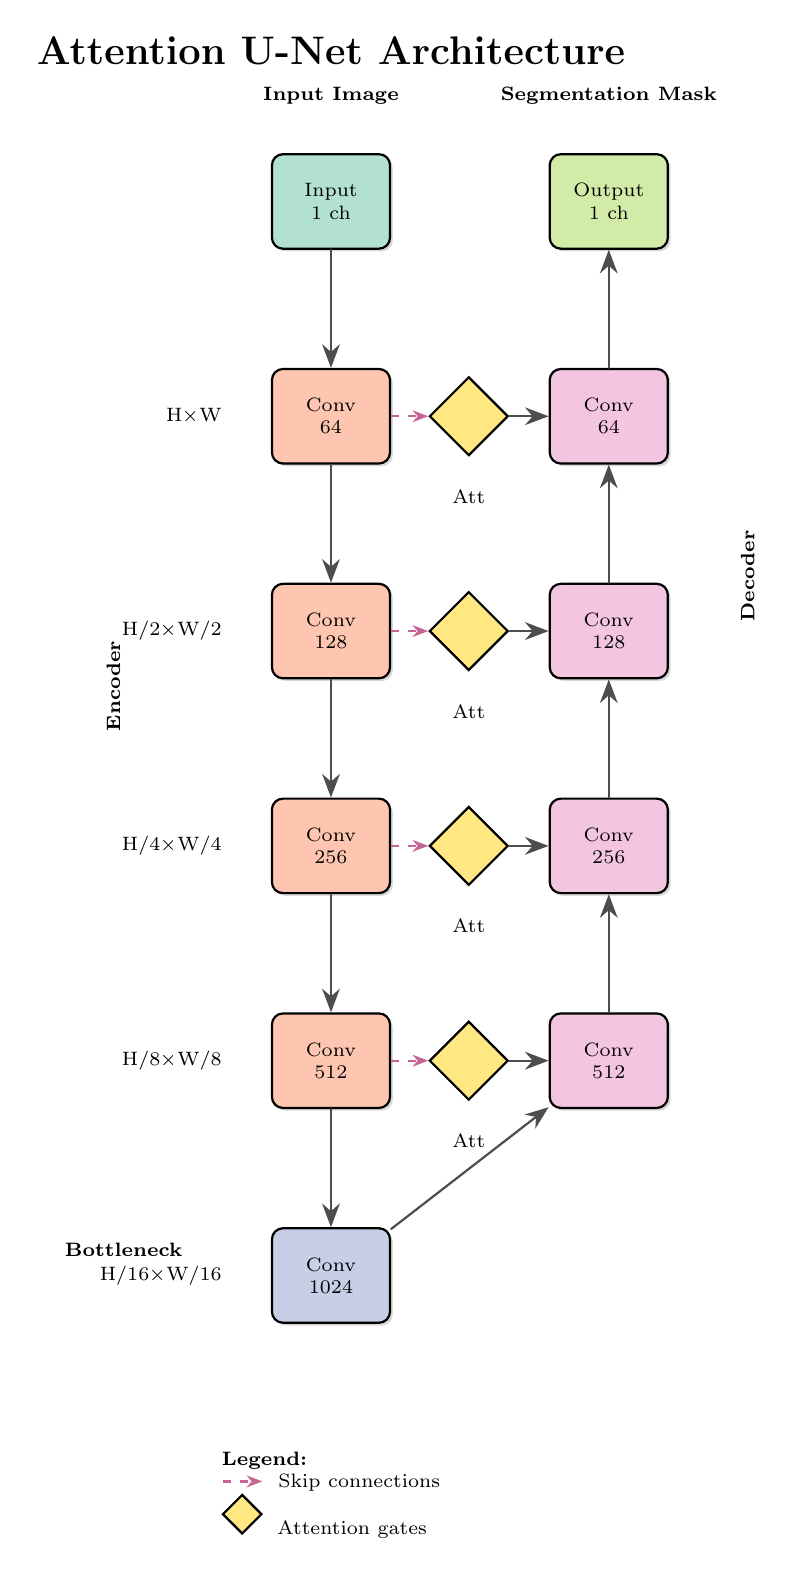
\begin{tikzpicture}[node distance=1.5cm and 2cm]

  % Input
  \node[convblock=inputcolor] (input) {};
  \node[smalltext] at (input) {Input\\1 ch};
  \node[smalltext, above=0.5cm of input] {\textbf{Input Image}};

  % Encoder path
  \node[convblock=encodercolor, below=of input] (enc1) {};
  \node[smalltext] at (enc1) {Conv\\64};
  
  \node[convblock=encodercolor, below=of enc1] (enc2) {};
  \node[smalltext] at (enc2) {Conv\\128};
  
  \node[convblock=encodercolor, below=of enc2] (enc3) {};
  \node[smalltext] at (enc3) {Conv\\256};
  
  \node[convblock=encodercolor, below=of enc3] (enc4) {};
  \node[smalltext] at (enc4) {Conv\\512};

  % Bottleneck
  \node[convblock=bottleneckcolor, below=of enc4] (bottleneck) {};
  \node[smalltext] at (bottleneck) {Conv\\1024};
      \node[smalltext, above left=-0.5cm and 1cm of bottleneck] {\textbf{Bottleneck}};

  % Decoder path
  \node[convblock=decodercolor, right=2cm of enc4] (dec4) {};
  \node[smalltext] at (dec4) {Conv\\512};
  
  \node[convblock=decodercolor, above=of dec4] (dec3) {};
  \node[smalltext] at (dec3) {Conv\\256};
  
  \node[convblock=decodercolor, above=of dec3] (dec2) {};
  \node[smalltext] at (dec2) {Conv\\128};
  
  \node[convblock=decodercolor, above=of dec2] (dec1) {};
  \node[smalltext] at (dec1) {Conv\\64};

  % Attention blocks
  \node[attention, left=0.5cm of dec4] (att4) {};
  \node[smalltext, below=0.3cm of att4] {Att};
  
  \node[attention, left=0.5cm of dec3] (att3) {};
  \node[smalltext, below=0.3cm of att3] {Att};
  
  \node[attention, left=0.5cm of dec2] (att2) {};
  \node[smalltext, below=0.3cm of att2] {Att};
  
  \node[attention, left=0.5cm of dec1] (att1) {};
  \node[smalltext, below=0.3cm of att1] {Att};

  % Output
  \node[convblock=outputcolor, above=of dec1] (output) {};
  \node[smalltext] at (output) {Output\\1 ch};
  \node[smalltext, above=0.5cm of output] {\textbf{Segmentation Mask}};

  % Encoder arrows (downsampling)
  \draw[arrow] (input) -- (enc1);
  \draw[arrow] (enc1) -- (enc2);
  \draw[arrow] (enc2) -- (enc3);
  \draw[arrow] (enc3) -- (enc4);
  \draw[arrow] (enc4) -- (bottleneck);

  % Upsampling arrows
  \draw[arrow] (bottleneck) -- (dec4);
  \draw[arrow] (dec4) -- (dec3);
  \draw[arrow] (dec3) -- (dec2);
  \draw[arrow] (dec2) -- (dec1);
  \draw[arrow] (dec1) -- (output);

  % Skip connections with attention
  \draw[skiparrow] (enc4) -- (att4);
  \draw[arrow] (att4) -- (dec4);
  
  \draw[skiparrow] (enc3) -- (att3);
  \draw[arrow] (att3) -- (dec3);
  
  \draw[skiparrow] (enc2) -- (att2);
  \draw[arrow] (att2) -- (dec2);
  
  \draw[skiparrow] (enc1) -- (att1);
  \draw[arrow] (att1) -- (dec1);

  % Side labels
  \node[rotate=90, smalltext, left=2cm of enc2] {\textbf{Encoder}};
  \node[rotate=90, smalltext, right=1cm of dec2] {\textbf{Decoder}};

  % Dimension annotations
  \node[smalltext, left=0.5cm of enc1] {H×W};
  \node[smalltext, left=0.5cm of enc2] {H/2×W/2};
  \node[smalltext, left=0.5cm of enc3] {H/4×W/4};
  \node[smalltext, left=0.5cm of enc4] {H/8×W/8};
  \node[smalltext, left=0.5cm of bottleneck] {H/16×W/16};

  % Title
  \node[above=1cm of input, font=\Large\bfseries] {Attention U-Net Architecture};

  % Legend
  \node[below=1.5cm of bottleneck, smalltext, align=left] {
    \textbf{Legend:}\\
    \tikz\draw[skiparrow] (0,0) -- (0.5,0); \ Skip connections\\
    \tikz\node[attention, minimum size=0.5cm]{}; \ Attention gates
  };

\end{tikzpicture}
\end{document} 